\documentclass[12pt]{article}
\usepackage{amsmath}
\usepackage{amssymb}
\usepackage{geometry}
\usepackage{enumerate}
\usepackage{float}%稳定图片位置
\usepackage{graphicx}%画图

\usepackage{wrapfig}
\usepackage{indentfirst}%缩进
\usepackage{enumerate}%加序号
\usepackage{multirow}%合并行
\usepackage{subfigure}
\usepackage{graphicx}
\title{\large UM-SJTU JOINT INSTITUTE\\Major Design Experience\\(VE450)\\\ 
\begin{figure}[H]
\centering
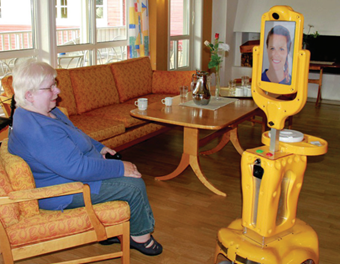
\includegraphics[scale=0.75]{P1.png}
\end{figure}
Design Review Report\\\  Telepresence Robot for Elderly\cite{1} \\\ \\\ Sponsor: JI CFE as part of mHBR initiative \\\ Mentor: Prof. Pradeep Ray, Prof. Artur Serrano \\\ Instructor: Prof. Guo Yunlong }
\author{
Pan Chongdan\qquad  panddddda@sjtu.edu.cn\\Boaro Fernando\qquad fernandoboaro21@sjtu.edu.cn
\\Liu Niyiqiu\qquad lnyq10@sjtu.edu.cn\\Qiu Tianyu\qquad qty2898734013@sjtu.edu.cn\\
Zhou Ruixing\qquad cncasper421@sjtu.edu.cn}
\date{Date: \today}
\begin{document}
\maketitle
\newpage
\section{Abstract}
\subsection{Project Motivation and Outcomes}
Telepresence robot for elderly people mainly aims at providing remote care for the elderly when their caregivers are far away from them. Indeed, telepresence robot can work as an alternative of personal visits and provide a real network of care. 
\par Nowadays, there are telepresence robots products used in Europe, and relative research shows they really increased elderly people's feelings of happiness, self-esteem and reduced their levels of frustration. However, they're too expensive and often difficult to operate due to a lot of limitations such as unstable network communication caused by firewall interruption. Therefore, we want to simplify and stabilize the robot so that the robot can be used by more people.
\par According to initial design, we want to realize stable remote control, visual communication and medicine dispensers. With such functions, the telepresence robot can thus maximize its value and provide emotional bonds between the elderly and caregivers. 
\subsection{Project Outcome}
A general image of our telepresence robot will be a tall touchscreen standing on a movable chassis. The core processor will be connected to the Internet so that  caregivers can control the robot remotely. The screen will be about 1 meter in height so that it's convenient for the elderly to watch. The robot will be within 0.6 meter in both length and width so that it can move indoors with flexibility. For safety, the robot won't be operated at voltage higher than 20V and there are less than 10 motors on the robot. The touchscreen will be about 7 inches on diagonal, which is enough to demonstrate a clear image within 1 meter's distance.
\subsection{Main Goals \& Challenges} 
\par The project includes following design goals and challenges:
\begin{enumerate}[-]
\item Designing, building and testing the robot under the cost of 1000 dollars.
\item Providing stable and instant remote communication with the elderly and caregivers 
\item Establishing a system stable enough for caregivers to control the movement of the robot in an easy way with the help from vision sensors.
\item Building medicine dispenser to distribute pills to the elderly as well as to notify them
\end{enumerate}
\subsection{General Project Plan}
We plan to build our first prototype before the end of October, then Pan Chongdan will communicate with our sponsors at Norway and get some feedback. In November, we will make adjustments to the robot according to the feedback.
\section{Introduction \& Problem Description }
With the acceleration of pace of life, people tend to spend more time away from home while leaving the elderly alone at home. Under this condition, on one hand, caregivers will be worried about old people's physical well-being, and on the other hand, without the connection with their family and children, the elderly will be more likely to feel lonely, which will further affect their mental health.\par
Telepresence robot is designed to cope with such scenario, with which caregivers are able to communicate and provide care with the elderly when they're away. From emotion perspective, the telepresence can also work as an substitute of the caregivers since it can enhance the connection between the elderly and their children.
\subsection{Problem}
\begin{wrapfigure}{r}{5cm}
	\centering
	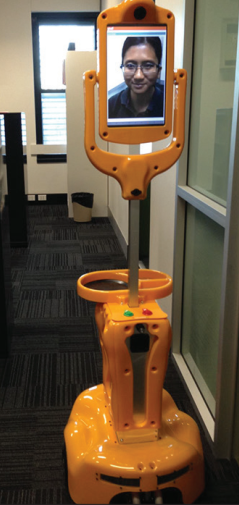
\includegraphics[scale=0.4]{P2.png}
	\caption{Giraffe robot\cite{1}}
	\label{fig::giraffe}
\end{wrapfigure}
\begin{enumerate}[1]
\item \textbf{Budget}
\par Our budget is under 1000 USD while similar products in the market is much more expensive than that (around 5000 USD), which means all structures and functions of the current version of robot cost too much. The most important problem for us is to redesign and simplify the robot to meet the goal of low budget. However, our robot should still be able to realize its essential function.
\item \textbf{Telepresence Technology}
\par The core technology of telepresence robot is to establish stable and simple connection between the operator and the robot. Since firewall exists and routers are often used at home, there are many obstacles impeding the transmission of control signal. What's more, since the caregivers need to take care of the elderly by robot at any time at any place, the control system based on portable devices becomes necessary.
\item \textbf{Stable Control System} 
\par In order to realize movement control between the caregivers and the robot, core processor, actuators and sensors are necessary. First, caregivers control actuators by giving instructions to the core processor connected the network. Then feedback will be given by sensors so that caregivers can know the status of the robot, which is important for further control. In this way, creating an integrated control system is also one of the most important tasks for our team.
\item \textbf{Functions for the elderly}
\par It's important to realize functions specially for the elderly. Since the elderly usually have distinct needs and  characteristics, the robot should be able to cope with different elderly people. For example. different old people need to take their own pills at different time, so the medicine dispenser must be flexible enough to coordinate with it. It should be able to dispense various pills at once.
\item \textbf{Safety and Power}
\par Since the elderly usually stay with the robot alone, safety is of high priority and the running voltage shouldn't be too high, which is less than 30 VDC. In addition, the robot should contain a battery of high capacity so that charge frequency can be reduced to avoid unexpected situations.
\end{enumerate}
\subsection{Competitive Products}
\subsubsection{Giraffe Telepresence Robot}
All the similar products in market right now is much more expensive than 1000 dollars, and the most representative product is \textbf{Giraffe} produced by a Europe company. The picture of a Giraffe robot is shown in Fig.~\ref{fig::giraffe}.
\textbf{Giraffe} has been put into the market for some time and it does have positive feedback on providing care and emotional connection to the elderly. However, it still has some problems such as firewall issues, video freezing, and driving lag etc, but it can be a reference based on which we can design and build our own telepresence robot.
\par In China typically, there is no such robotic products. The most similar products would be some smart furniture.
\subsection{Relevant Hardware \& Software}
\subsubsection{Raspberry Pi}

\begin{figure}[H]
	\begin{minipage}[t]{0.5\linewidth}
		\centering
		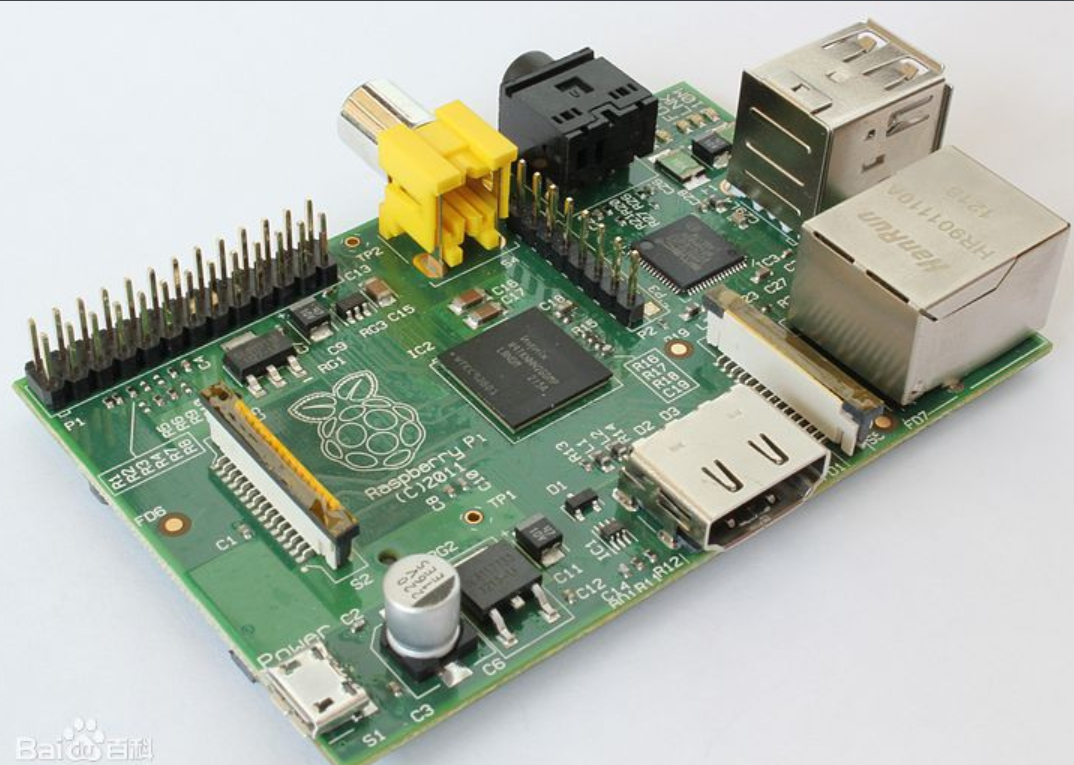
\includegraphics[width=2.2in]{P3}
		\caption{Central processing Board\cite{8}}
		\label{fig::relevent::pi}
	\end{minipage}%
	\begin{minipage}[t]{0.5\linewidth}
		\centering
		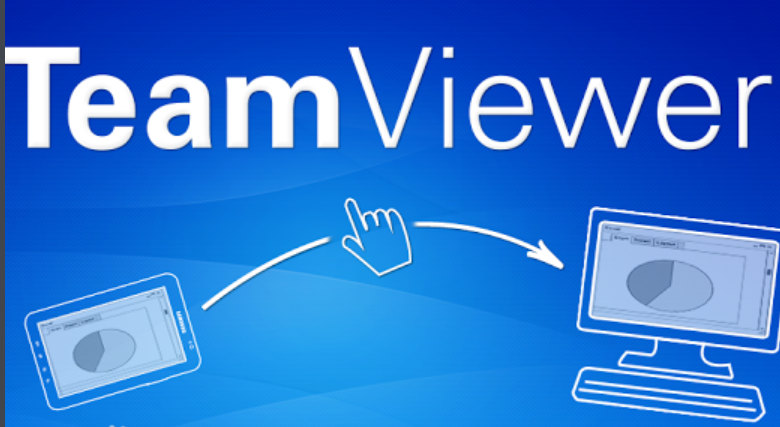
\includegraphics[width=2.4in]{P4}
		\caption{Software for Remote Control\cite{9}}
		\label{fig::relevent::teamviewer}
	\end{minipage}
\end{figure}
Raspberry Pi is a micro computer with many I/O interface so that it's easy for us to develop and control functions based on it. The operating system for Raspberry Pi is Linux. Python scripts can be written to realize Internet connection. Raspberry Pi can be a good central processing unit for telepresence robot. The size of a Raspberry Pi is very small, as shown in Fig.~\ref{fig::relevent::pi}. It can be fit into our telepresence robot occupying very little volume.
\subsubsection{Team Viewer}
Team Viewer is a software developed in Germany which can provide stable remote control between different computers. What's more, team viewer can be applied on any devices connected to World Wide Web as long as it has its own operating system. Team viewer makes it possible to realize stable remote control on portable devices.
\subsubsection{Screen, Camera, Actuators and Sensors}
A big touchscreen is connected to the raspberry pi. With this screen, the elderly can have visual communications with caregivers freely. On the other hand, camera like OpenCV can get pictures from the elderly or the surrounding environment for caregivers, so that they can control the robot and contact the elderly more easily. Actuators and sensors will play an auxiliary role to realize such functions, and be responsible for the movement of our robot.
\section{Information Sources}
\subsection{Medicine Dispenser}
\subsubsection{Background}
More than 50\% of the older people are living with multiple chronic illnesses\cite{2}. Thus, routine monitoring and assessment of the individual’s adherence is crucial to improve their health outcomes. Elderly with multiple chronic conditions face the complex task of medication management that can involving multiple medications of varying doses at different times. Advances in tele-health technologies have resulted in home-based devices for medication management and health monitoring for the elderly\cite{3}. The function of such medication dispensers is to alert the patient when it is the date and time to take their prescribed medication\cite{4}. When the time comes to take the medication, the pill dispenser automatically releases a pre-measured dose for consumption.
\subsubsection{Medicine Dispenser Standards\cite{5}}
\begin{itemize}
    \item Provides audible, visible or vibration alerts.
    \item Dispenser must be locked once medicine is replenished.
    \item Long distance connectivity to track use.
    \item Humidity resistant and tamper proof.
    \item Dispense only the prescribed amount at the required times.
\end{itemize}
\subsection{Telepresence Robot}
\subsubsection{Telepresence Robot Standards}
Telepresence Robots are a very new and unique type of robot in the market nowadays, and since there are standards for collaborative industrial robots (Cobots) and AGVs (automated guided vehicles) our robot would not be included in such standards because 1) Our robot does not include a robotic arm so it is not considered an collaborative industrial robot and 2) Since our telepresence robot will be a simplified version of our competitors due to our budget restriction, we will not be adding any obstacle avoidance sensors, instead, the person controlling the robot is responsible for its movement, thus it cannot be considered and neither can AGVs. The standards we have to abide by will therefore be our electronic components such as battery and CPU, but since we will buy our batteries and CPU from third party manufacturers (already passed safety regulations and standards) we will not have to worry about any hazard as long as we use the equipment correctly according to the manufacturers.

\section{Custom Requirements and Engineering Specifications}
The custom requirements of our project are divided into the software and hardware part. They are summarized as follows:
\subsection{Hardware Standard}
\begin{enumerate}
	\item The screen, along with its control buttons, should be large enough 
	\item The speaker should be loud enough for the elderly 
	\item The height of the screen should be suitable for old people who sit in a chair to watch 
	\item The medicine dispenser should be located on a suitable height 
	\item The medicine dispenser should have large storage 
	\item The medicine dispenser should provide dry environment to store the medicines
	\item The moving speed of the chassis should not be too fast or too slow
	\item The battery duration of the robot should last a long time 
	\item The physical entity of the robot does not contain any sharp edges 
\end{enumerate}
\subsection{Software Standard}
\begin{enumerate}
	\item Control (both local and remote) of the robot should be easy 
	\item Has alarm function to remind the elderly to take medicines
	\item Has auto obstacle detection and evasion algorithm 
\end{enumerate}

Besides these requirements from the two aforementioned categories, the total cost of the robot should be below 1000\$.

Considering the robot itself, we separate the robot into the following four functional parts: 1) Chassis of the robot, 2) Medicine Dispenser, 3) Touchscreen \& camera, 4) Raspberry Pi controller. The generated engineering specifications, along with the custom requirements are shown in Fig.~\ref{fig::qfd}.

\begin{figure}[H]
	
	\centering
	\includegraphics[width=7in]{qfd}
	\caption{QFD table of our project.}
	\label{fig::qfd}

\end{figure}
   In Fig.~\ref{fig::qfd} above, we list 12 customer requirements and 10 engineering specifications, rate their relationships, and calculate the priority. Each strong relationship counts 9 points, each moderate relationship counts 3, and each weak relationship counts 1. Multiply by the importance points of the requirements, we can calculate the weighted average of each specification. The specification with highest weight has the highest priority. We found out that the remote control lag is the most important one, and the motor power and the weight follow. The least important one is the dB of the speaker. Tab.~\ref{tab:spec} shows the details of the specifications.
   
\begin{table}[H]
	\centering
\begin{tabular}{|c|c|c|c|}
\hline
Specs. & Speaker Loudness(dB)   & Battery Vol.(mAh) & Screen Resol.(Pixels)   \\ \hline
Target   & 80                     & 20000               & 1280*720                    \\ \hline
Specs. & Motor Power(W)         & Cost(RMB)           & Med. Storage Volume(mL) \\ \hline
Target  & /                      & 5000                & 100                         \\ \hline
Specs. & Yeild Strength(MPa)    & Weight(g)           & Camera Pixel(Pixels)        \\ \hline
Target   & /                      & 5000                & about 500,0000              \\ \hline
Specs. & Remote Control Lag(ms) &                     &                             \\ \hline
Target    & 10                     &                     &                             \\ \hline
\end{tabular}
\caption{Engineering specifications of our design }
\label{tab:spec}
\end{table}

\section{Project Plan}
\subsection{Project Milestone \& Gantt Chart}
Three students major in ECE and two students major in ME form our group. Considering team members' specialties, our project is mainly divided into ME part and ECE part.\par 
ME part concerns mostly the hardware of the robot (Fig.~\ref{fig::megantt}). Fernando and Ruixing are mainly in charge of designing and building medicine dispenser, fall detector and assembling and testing the robot.\par
\begin{figure}[H]
	
	\centering
	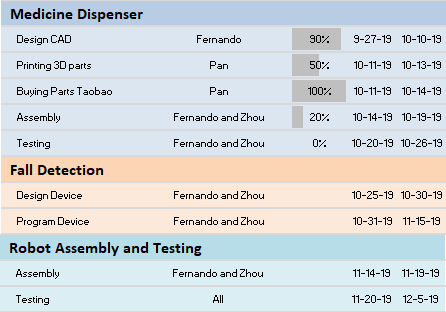
\includegraphics[width=3in]{ganttA.png}
	\caption{ME Gantt Chart}
	\label{fig::megantt}

\end{figure}
ECE part mainly consists of robot movement control, function implementation and user interface design (Fig.~\ref{fig::ecegantt}). Chongdan and Niyiqiu are mainly in charge of user interface design. Niyiqiu and Tianyu are in charge of function implementation, and Chongdan and Tianyu are in charge of the circuit design of the robot.
\begin{figure}[H]
	
	\centering
	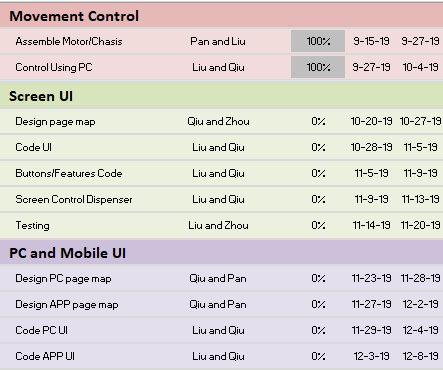
\includegraphics[width=3in]{ganttB.png}
	\caption{ECE Gantt Chart}
	\label{fig::ecegantt}

\end{figure}
From our complete Gantt chart in Fig.~\ref{fig::gantt}. we can see the groups progress with our tasks. We are prioritizing the robots functionality such as smooth movement, medicine dispenser and fall detection, therefore these tasks are towards the earlier weeks. While our user friendly interface although very important is left for the later weeks since it is not an integral part of the project.
Our progress so far has been acceptable, although we are a little behind schedule with the medicine dispenser, movement control has been completed and we are satisfied with the results. We are also getting ready to start work on our screen UI and fall detection tasks. We should have no problem in being able to deliver a finished product with all its working specifications by the end of the semester.
\begin{figure}[H]
	
	\centering
	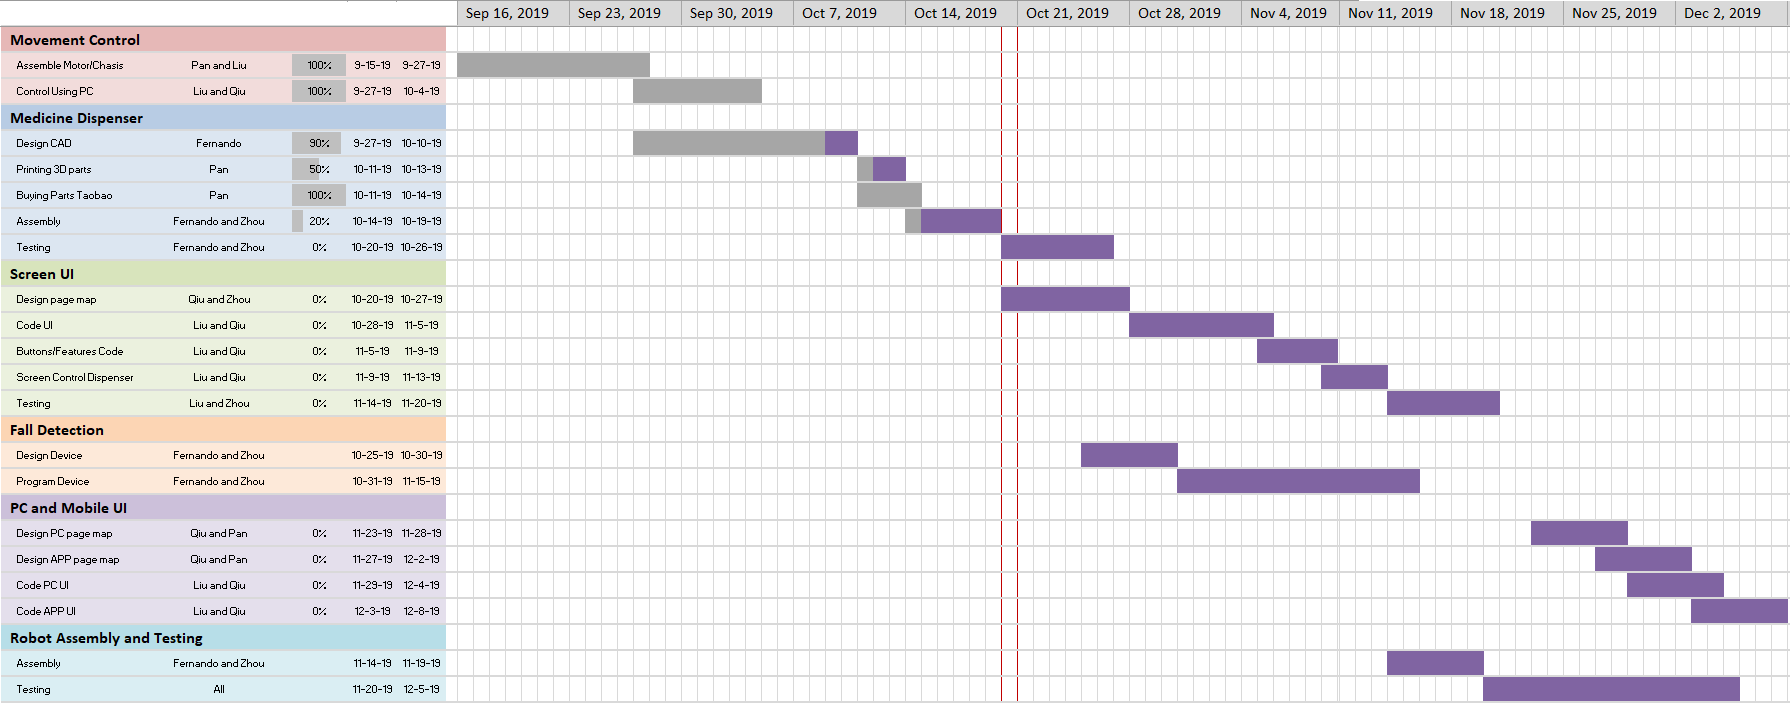
\includegraphics[width=6in]{ganttC.png}
	\caption{Gantt Chart}
	\label{fig::gantt}

\end{figure}
\subsection{Project Budget}
\begin{figure}[H]
	
	\centering
	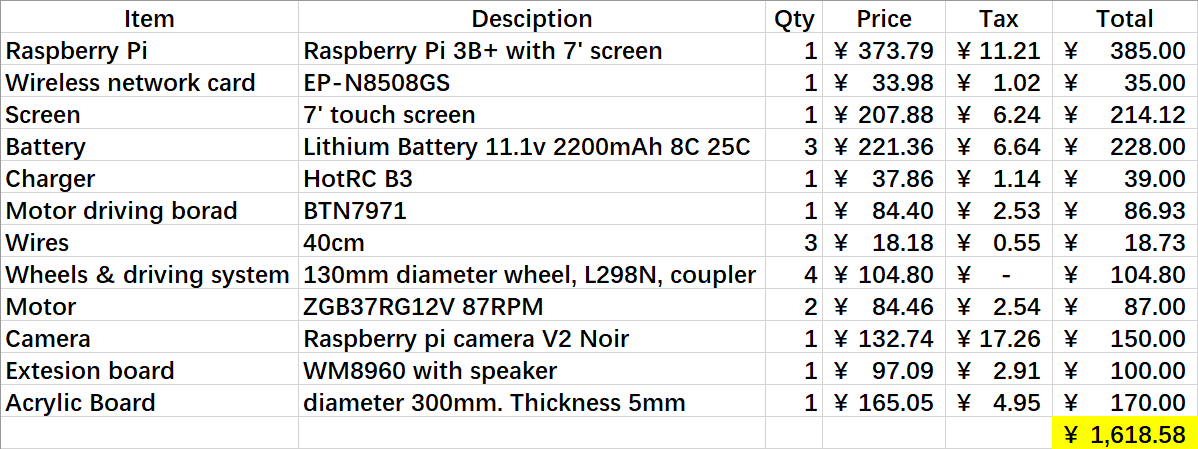
\includegraphics[width=6in]{budget.png}
	\caption{Project Budget}
	\label{fig::gantt}

\end{figure}
The table above lists what we have already spent on our project. Raspberry Pi really reduce the cost to a great extent and the main structure of medicine dispenser is 3D printed. This table will be updated as soon as more items is needed. Currently the overall budget is well under control.


\section{Conclusion}
Telepresence robots are still a relatively new technology in which a person can transmit his “presence” by controlling a robot with his projection on a screen, the idea is that someone can be “present” in the room even though they are located anywhere in the world. Telepresence robots can be particularly useful for elderly care, where family members can control the robot and give attention to the elderly on a more regular basis, with additional functions such as being able to monitor the medication intake and being alerted when a fall has been detected. Thus the elderly do not necessarily have to move to elderly care homes, instead they can remain in the comfort of their homes while still receiving the proper attention and care necessary.\par
However, current telepresence robots for the elderly are expensive according to the users\cite{6} , around 5 to 15 thousand dollars for a model, the persistent connectivity issues also make it hard to operate and control, causing a negative feedback from the elderly and caretakers alike\cite{7}.\par
Our goal for this project is to design and build a telepresence robot for the elderly that has a desirable price point of less than 1 thousand dollars, and while maintaining the features such as medicine dispenser and fall detection, we would also improve the connectivity issue to ensure a better and complete user experience.
\newpage
\begin{thebibliography}{99}
\bibitem{1} Donald Kerr, J Artur Serrano, Pradeep Ray, “ The role of a disruptive digital technologyfor home‑based healthcare of the elderly: Telepresence robot ,"  Digital Medicine, Year 2018, Volume 4, Issue 4 [p. 173-179]
\bibitem{8} https://gss2.bdstatic.com/-fo3dSag\_xI4khGkpoWK1HF6hhy/baike/crop\%3D40\\\%2C0\%2C717\%2C474\%3Bc0\%3Dbaike92\%2C5\%2C5\%2C92\%2C30/sign=c27ab\\7a130292df5838cf65581056c4c/9358d109b3de9c8287cc8b016681800a18d84396.jpg
\bibitem{9} https://gss1.bdstatic.com/9vo3dSag\_xI4khGkpoWK1HF6hhy/baike/crop\%3D56\\\%2C0\%2C520\%2C343\%3Bc0\%3Dbaike80\%2C5\%2C5\%2C80\%2C26/sign=f63045\\cb3ffae6cd18fbf12132863908/78310a55b319ebc4d65ed2658826cffc1e171623.jpg
\bibitem{2} Yap, A.F.; Thirumoorthy, T.; Kwan, Y.H. Systematic review of the barriers affecting medication adherence in older adults. Geriatr. Gerontol. Int. 2016, 16, 6993–7001.
\bibitem{3} Reeder, Blaine, et al. “Older Adults' Satisfaction with a Medication Dispensing Device in Home Care.” Informatics for Health & Social Care, U.S. National Library of Medicine, Sept. 2013, www.ncbi.nlm.nih.gov/pmc/articles/PMC4122419/.
\bibitem{4} Sumo Guide. “Best Automatic Pill Dispenser - Top 10 Reviews 2019.” Sumo Guide | The Ultimate Shopping Guide & Product Reviews, Sumo Guide Team Https://Sumoguide.com/Wp-Content/Uploads/2016/09/Sumo-Guide-Logo-300x100.Png, 31 July 2019, sumoguide.com/best-automatic-pill-dispenser-reviews/.
\bibitem{5} American Society of Health-System Pharmacists. ASHP guidelines on the safe use of automated dispensing devices. Am J Health-Syst Pharm. 2010; 67:483–90.
\bibitem{6} Reeder, Blaine, et al. “Older Adults' Satisfaction with a Medication Dispensing Device in Home Care.” Informatics for Health & Social Care, U.S. National Library of Medicine, Sept. 2013, www.ncbi.nlm.nih.gov/pmc/articles/PMC4122419/
\bibitem{7} Donald Kerr, J Artur Serrano, Pradeep Ray, “ The role of a disruptive digital technology
for home based healthcare of the elderly: Telepresence robot ,"  Digital Medicine, Year 2018, Volume 4, Issue 4 [p. 173-179]



\end{thebibliography}
\newpage
\section*{Bios}
\subsection*{Chongdan Pan}
\begin{figure}[H]
    \centering
    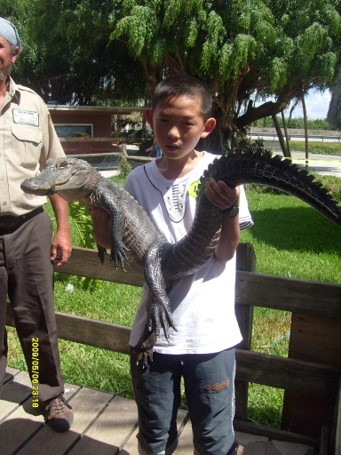
\includegraphics[width=2in]{p.jpg}
    \caption{Chongdan Pan}
    \label{fig::pan}
\end{figure}
Pan, Chongdan is a senior student major in electronic and computer engineering. He has gathered some experience in robotic field by participating a few robotic competitions. He has won an Asia champion and world champion in VEX robotic championship, and he will continue to study robots in the future. Now, he is applying for graduate programs related in computer engineering and robotics in the United States. In our project, he is mainly responsible for overall design and providing sources like tutorial or 3D print.
\subsection*{Fernando Boaro}
\begin{figure}[H]
    \centering
    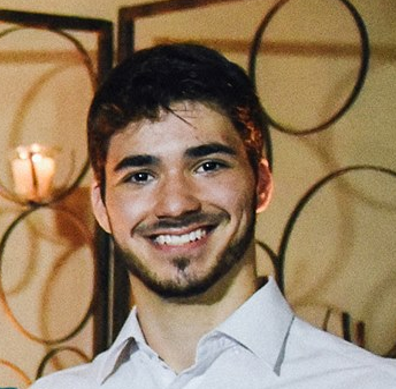
\includegraphics[width=2in]{f.png}
    \caption{Fernando Boaro}
    \label{fig::fer}
\end{figure}
Fernando Boaro is an undergraduate student completing his Mechanical Engineering studies in Shanghai Jiao Tong University, with an expected graduation on March, 2020. Fernando has completed two internships during his time at Jiao Tong, spending three months in Flieden, Germany as a mechanical engineering intern at A.I.C. RobotiX UG, a robotics startup company focusing on warehouse robots, where his main tasks were research and development and CAD design. And in 2019 completing another three month internship as a mechanical engineering intern at Mikron Industrial Automation in Shanghai, China, where his main tasks were the redesign of a protective machine door and designing CAD parts for customer projects. After his university studies Fernando plans to move to Germany and work as a mechanical engineer in the industrial robot industry.
\subsection*{Niyiqiu Liu}
\begin{figure}[H]
    \centering
    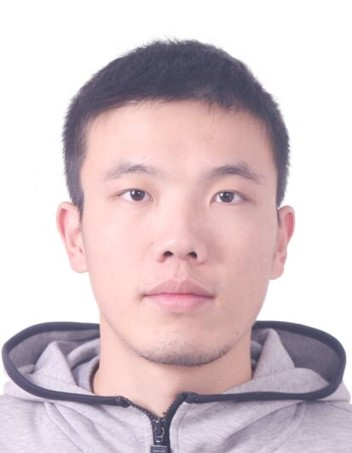
\includegraphics[width=2in]{l.jpg}
    \caption{Niyiqiu Liu}
    \label{fig::liu}
\end{figure}
Liu Niyiqiu is a senior student major in ECE. He is now following the computer science track in the ECE degree and is applying for graduate programs in the United States. He is in charge of software side of the project.
\subsection*{Ruixing Zhou}
\begin{figure}[H]
    \centering
    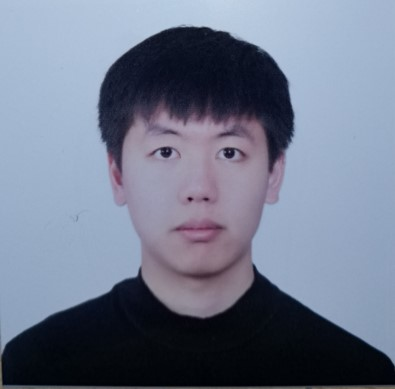
\includegraphics[width=2in]{z.jpg}
    \caption{Ruixing Zhou}
    \label{fig::qiu}
\end{figure}
Zhou Ruixing, a senior student major in ME, is focusing on the manufacturing area in the mechanical engineering degree. He has a good knowledge in engineering design and is well-experienced in CAD drawing. He is responsible for the structure design & manufacture part of this project.
\subsection*{Tianyu Qiu}
\begin{figure}[H]
    \centering
    
\includegraphics[width=2in]{q.jpg}
    \caption{Tianyu Qiu}
    \label{fig::qiu}
\end{figure}
Qiu Tianyu is a senior student major in ECE. He has great interest in circuit design and control system and is applying for graduate programs in the United States in Electrical Engineering. He is in charge of coding and circuit design in the project.
\end{document}